% !TeX root = ../main.tex

\section{Simulación y análisis}

\subsection{Eventos}
Nuestro modelo tiene la característica de alimentarse de
datos externos para simular los efectos climáticos en la generación de
energía, y las variaciones en el consumo de un hogar. Es por eso, que en vez
de utilizar datos producidos aleatoriamente exclusivamente para llevar a cabo
este trabajo, optamos por utilizar fuentes de datos disponibles en internet,
pero que corresponden a casos reales.

En primer, como fuente de datos de clima, utilizamos un dataset de
Kaggle\footnote{\url{https://www.kaggle.com/runphilrun/hi-seas-solar-radiation-prediction}},
una plataforma para abierta para compartir fuentes de datos, y llevar a cabo
competencias en ciencias de datos. Los mismos fueron recolectados por
NASA\footnote{\url{https://hi-seas.org/}}, en dos misiones llevadas a cabo en
una instalación ubicada en la base de un volcán en Hawaii, Estados Unidos. La
expedición es llamada HI-SEAS (\textit{Hawai’i Space Exploration Analog and
Simulation}), y los datos corresponden a las misiones IV y V (septiembre a
diciembre de 2016).

La fuente de datos posee diversas mediciones meteorológicas, pero de estas
solo nos interesa la radiación solar, medida en $\frac{Watts}{m^2}$; y la
velocidad del viento, medida en $\frac{km}{hora}$. Todas estas mediciones
fueron realizadas con una frecuencia de cinco minutos.

Por otro lado, la fuente de datos utilizada para el consumo eléctrico
corresponde a \textit{University of California,
Irvine}\footnote{\url{https://archive.ics.uci.edu/ml/datasets/Individual+household+electric+power+consumption}},
y fueron tomadas en una casa en Francia, entre diciembre de 2006 y 2010. El
dato que extrajimos de esta fuente es la potencia activa consumida, medida
cada un minuto, y cuya unidad es $Watts$. Algo importante a notar, que puede
ser posible gracias a la asincronía que soporta DEVS en los eventos que
suceden, es que $1,25\%$ de las mediciones son nulas (debido a algún
inconveniente en la lectura de las mismas), las cuales fueron omitidas, y por
consiguiente, no incluidas entre los eventos disparados en la simulación.

Los eventos fueron procesados y combinados en un solo archivo de eventos. El
procesamiento consistió en: 
\begin{itemize} 
    \item Conversión de las unidades originales de las fuentes de datos a las
    utilizadas en el modelo.
    \item Normalización de las fechas asignadas a cada medición, para que las
    mismas arranquen en 00:00:00:00 (en tiempo DEVS, el inicio de la
    simulación), y conversión de las mismas al formato de tiempo utilizado
    por el simulador, respetando la diferencia relativa entre los eventos.
    Para esto se tomo la fecha 00:00:00:00 como la hora 00:00 AM, del primer
    día simulado.
    \item Inclusión de ambas fuentes de datos en un mismo archivo de eventos.
    Resultó interesante descubrir que el simulador ignora el orden en el que
    lee los eventos del archivo, ya que después al programarlos para ser
    disparados los reordena, lo cual permite armar el archivo no teniendo que
    ordenar los eventos manualmente.
\end{itemize} % TODO: Descripción cuantitativa de los datos?

\subsection{Elección de generadores}
Para calcular la energía generada por la celda solar, usamos la siguiente formula:

$$producedEnergy = \frac{radiation \times PeakPower \times Area}{1000}$$

Donde $PeakPower$ es un factor que depende del generador.

Buscamos las especificaciones de un equipo\footnote{https://www.fiasa.com.ar/DoWNloADs/FIASA-FOLLETO-GENERADOR-SOLAR.pdf}  
y tomamos uno con $PeakPower=100$. Consideramos entonces un panel solar de 1m$^2$ y con estos valores calculamos la
energía producida por este medio.

Para la turbina eólica buscamos un modelo teórico que explique los valores generados,
pero no lo pudimos ajustar con las especificaciones de turbinas, así que elegimos un
modelos y utilizamos una interpolación de manera que se ajuste a los valores 
provistos por el vendedor. \footnote{https://articulo.mercadolibre.com.ar/MLA-616433420-turbina-generador-eolico-aerogenerador-1200w-48v-enertik-\_JM}

\subsection{Ambiente de Simulación y experimentación} 
El procedimiento que utilizamos para llevar a cabo la simulación y analizar
los datos, consiste en, teniendo el archivo con los eventos procesados,
simular la cantidad de tiempo deseada (una semana en la mayor parte de los
análisis). Luego, utilizando los resultados obtenidos de la simulación
(puertos de salida del \textit{top model}, y logs (no propios de DEVS, sino
instrumentados en el modelos en si) obtenidos de alguna de los modelos), se
realizó un análisis cuantitativo y cualitativo.

Para el análisis de los datos, se utilizo \textit{Jupyter Notebooks}, junto
con diversas bibliotecas de \textit{Python}, tanto para lectura, filtrado y
transformación de los datos; como para graficar y obtener medidas
estadisticas.

\subsection{Desarrollo}
El desarrollo esta organizado de la manera en la que fueron sucediendo las
simulaciones realizadas (se incluye en cada una las configuraciones pasadas
al simulador, de forma de poder replicarlas fácilmente\footnote{Todos los
comandos son tomando como directorio base:
\textit{TP\_ROOT/simulation/src}.}; y el correspondiente \textit{notebook}
con el análisis). Cada sección tiene algunas conclusiones parciales, y
construye sobre la anterior.

\subsubsection{¿Cuál medio de generación aporta más?}
% ./bin/cd++ -e../eventGeneration/mergedData.ev -mmodels/solarAndWindControllerModel.ma -oout/solarAndWind1Week -lout/solarAndWind1Week.log -t168:00:00:00



\subsection{Consumo acumulado:}
A continuación observaremos las señales enviadas desde el controlador a la red, graficando
como positivas las señales de pedido de energía por parte de la red, y como negativas las
de venta de energía a la red.

El tiempo considerado es de una semana y la energía solicitada/pedida se mide en Watts hora.

\begin{figure}[H]
    \centering
    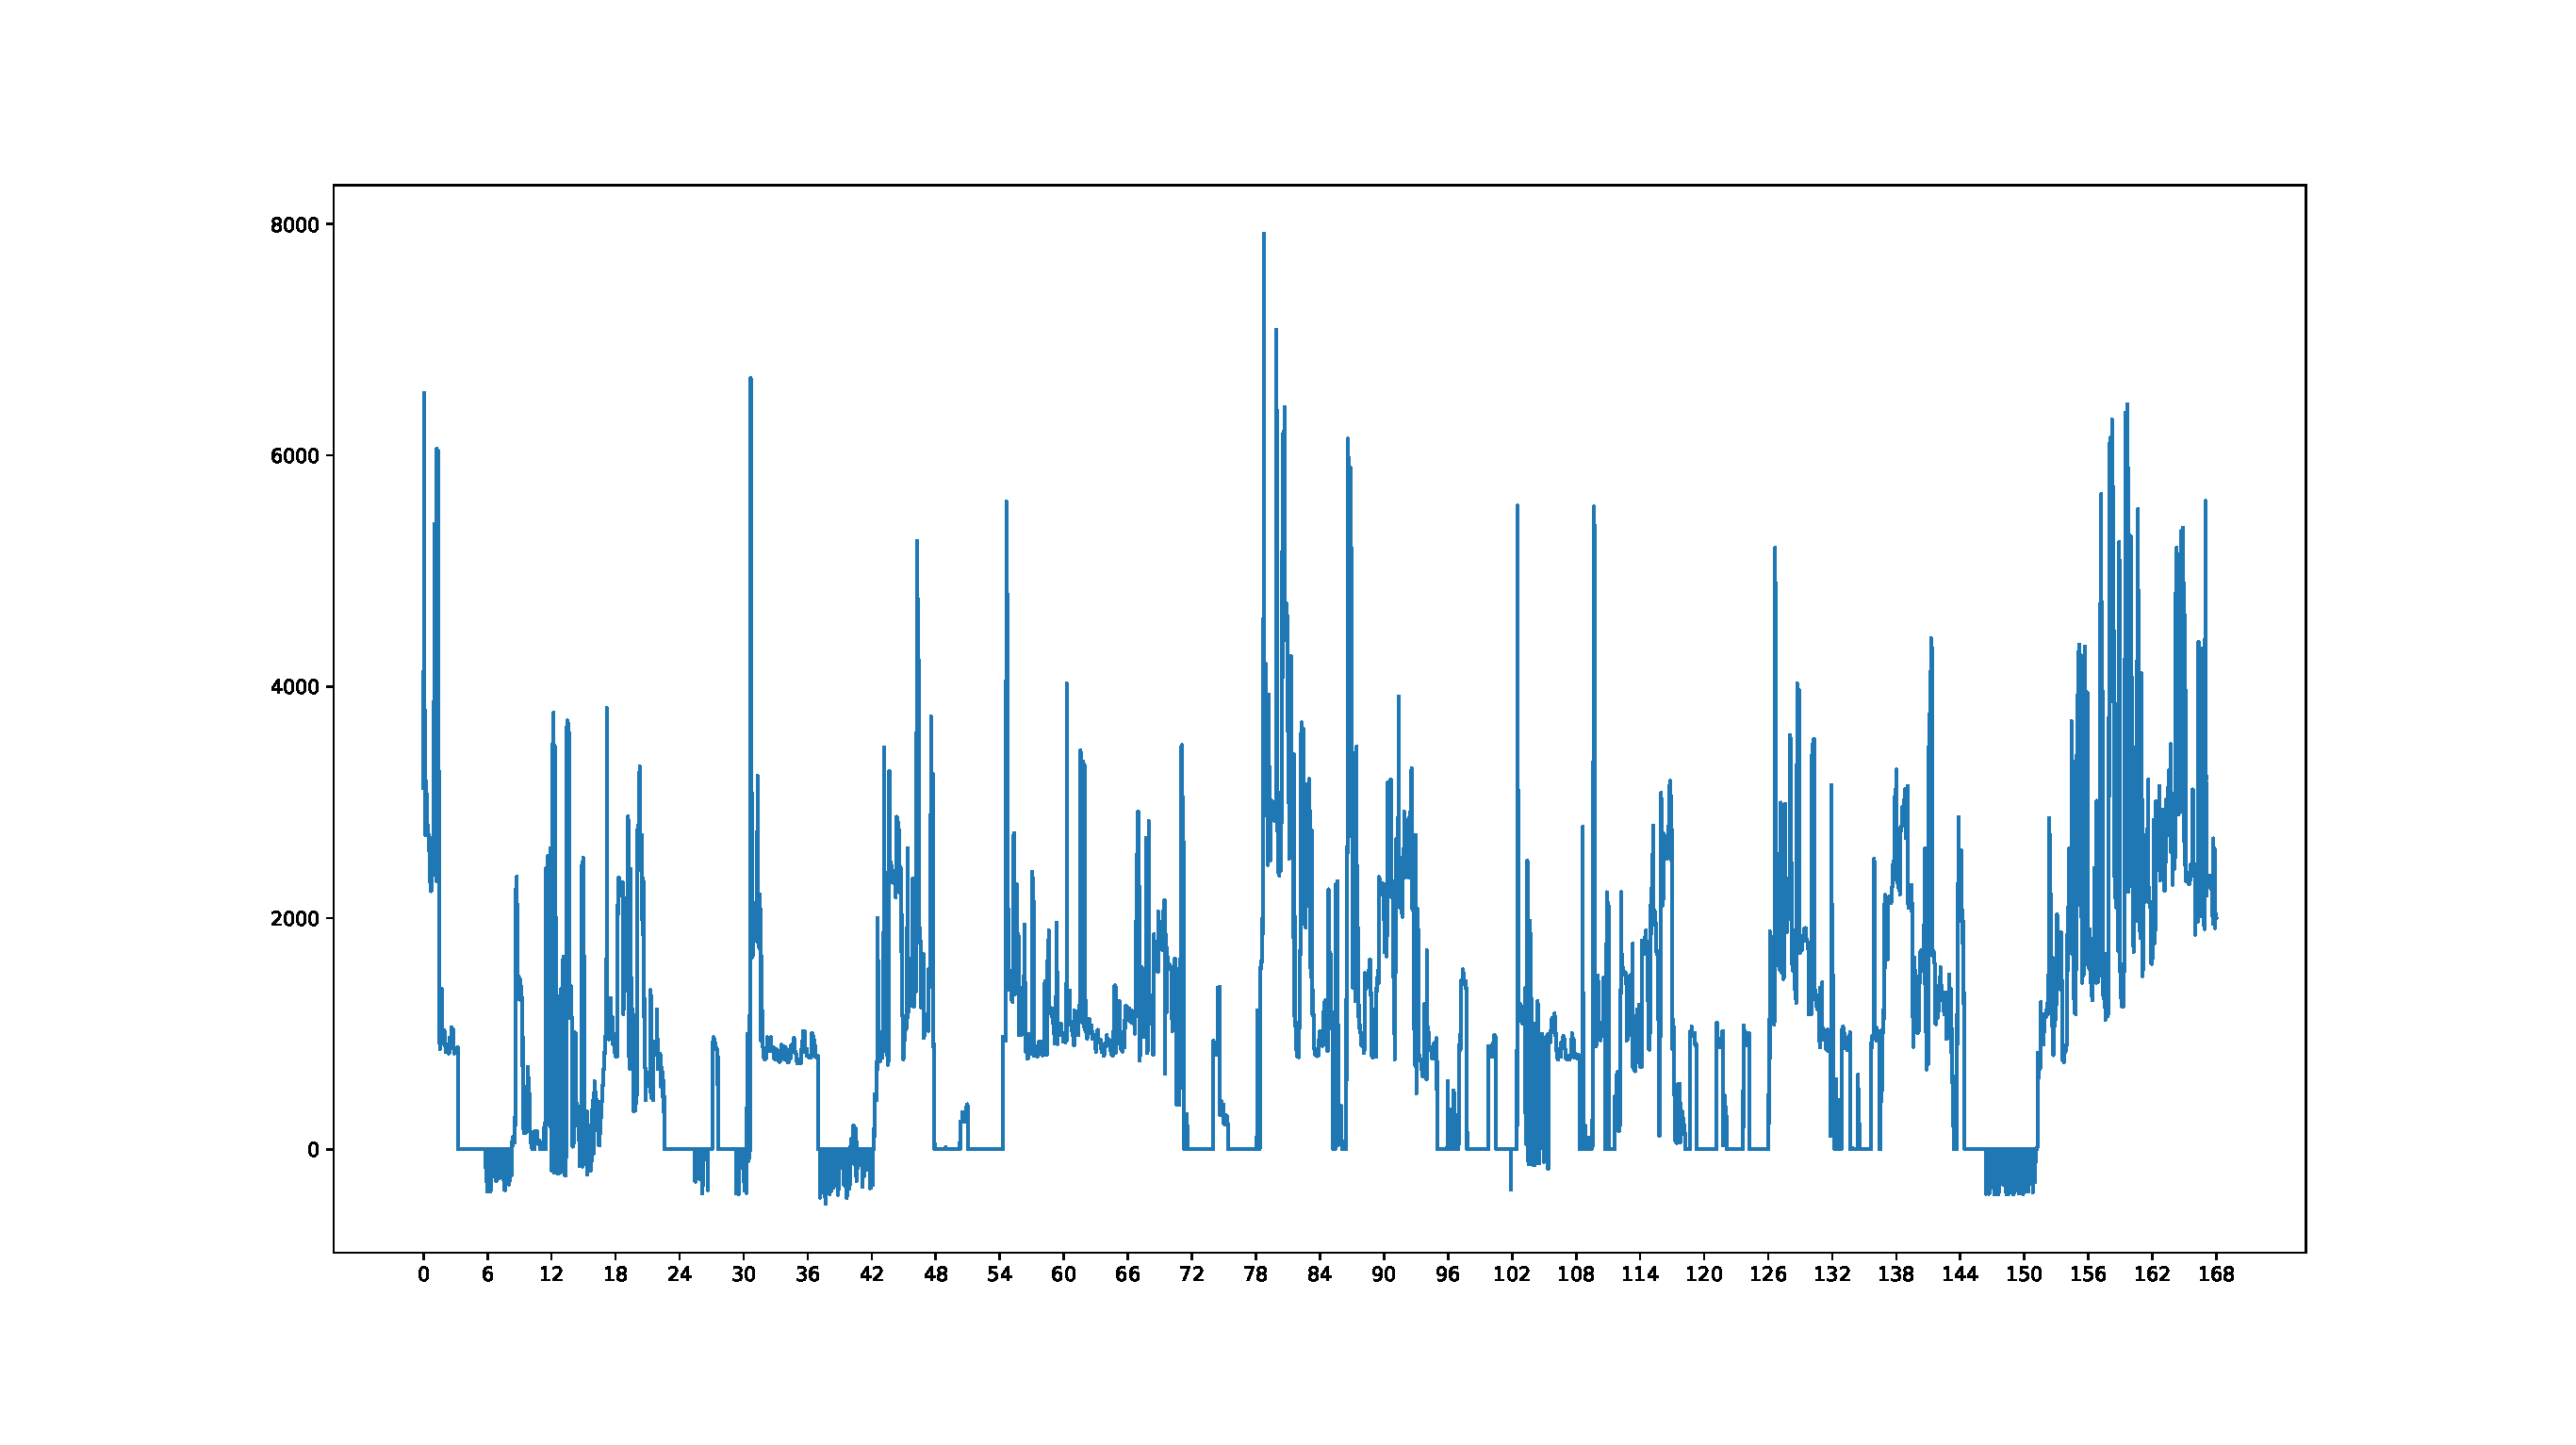
\includegraphics[scale=0.3]{images/cons.eps}
\end{figure}

Ahora calculamos el acumulado de estos valores podemos observar como evoluciona el
balance de energía. 

\begin{figure}[H]
    \centering
    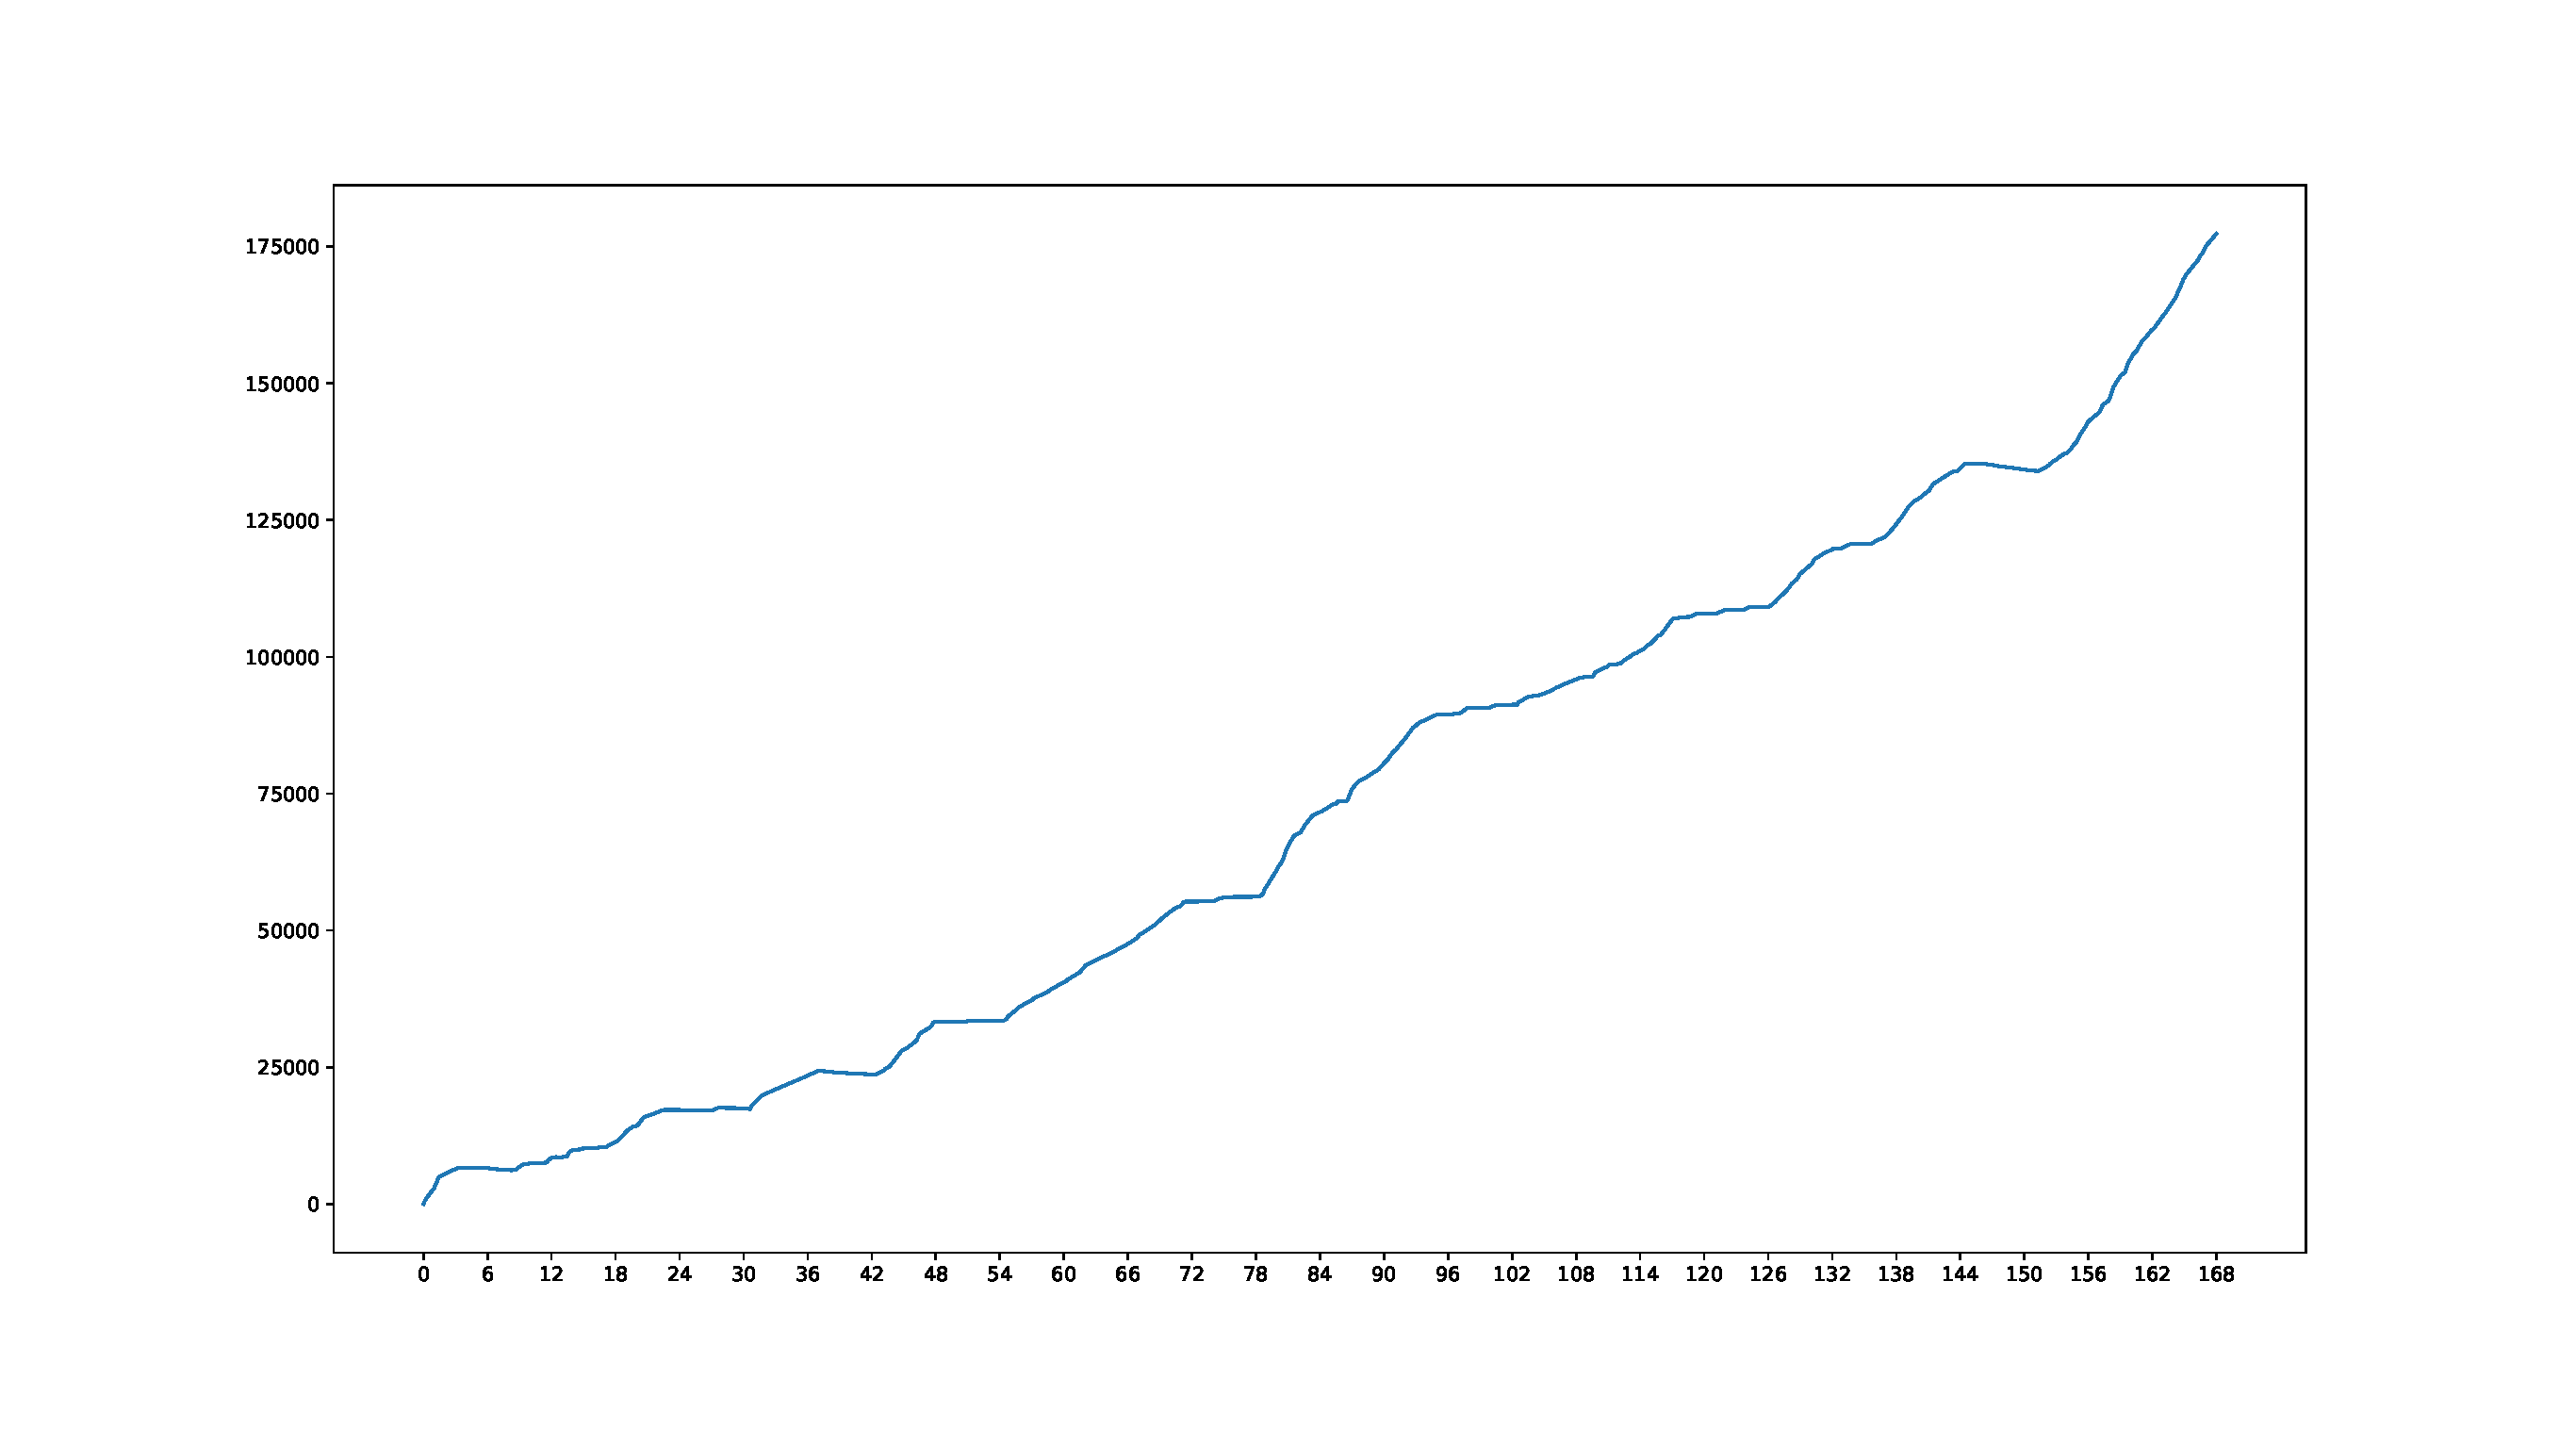
\includegraphics[scale=0.3]{images/acc.eps}
\end{figure}

En el gráfico vemos que con estos generadores aún existe bastante dependencia de la red,
pero el consumo de una semana es mucho menor (175kW).